\chapter{Analisis}
\label{chap: Analsisis}

Berdasarkan hasil studi pustaka yang telah dilakukan, pada bab ini akan dijelaskan hasil analisis
yang berupa spesifikasi dari perangkat lunak, diagram use-case, skenario.

\section{Analisis Perangkat Lunak yang Dibangun}
\label{sec: Analisis Perangkat Lunak yang Dibangun}
Dari pengetahuan yang diperoleh melalui studi pustaka yang dilakukan. Telah ditentukan beberapa analisis untuk membangun Perangkat Lunak Pohon Kurikulum 2018 menggunkan JSON. Berikut beberapa analisis yang telah diambil dari bab 2: 
\begin{itemize}
\item \textbf{Menggunakan \textit{JSON} yang konversikan ke dalam \textit{DOT Language}}
Untuk membuat graf harus dilakukan konversi dari\textit{JSON} ke dalam \textit{DOT Language}. \textit{DOT Language} sendiri digunakan untuk menghasilkan graf yang akan menampilkan pohon kurikulum. 

\item \textbf{\textit{JSON} dipakai sebagai data terbuka}
\textit{JSON} akan di simpan di \url{github.com}. Tujuannya agar \textit{JSON} menjadi format data terbuka. Setelah disimpan di dalam \url{github} \textit{JSON} dapat dipakai oleh siapa saja. Karena \textit{github} sendiri merupakan \textit{open source}.

\item \textbf{Perangkat Lunak Menghasilkan Graf Berbentuk Pohon Kurikulum}
Perangkat lunak yang akan dibangun akan menghasilkan graf yang berbentuk pohon kurikulum. Pohon kurikulum ini diperlukan agar mahasiswa mengetahui mata kuliah yang akan di ambil di semester baru. 

\item \textbf{Perangkat Lunak akan Menampilkan Mata Kuliah}
Perangkat Lunak yang dibangun setelah menghasilkan pohon kurikulum akan menampilkan mata kuliah yang ada di kurikulum baru. Mata Kuliah akan berisi mata kuliah wajib, mata kuliah pilihan, dan mata kuliah pilihan wajib.
\end{itemize}

\section{Spesifikasi Perangkat Lunak yang Dibangun}
\label{sec: Spesifikasi Perangkat Lunak yang Dibangun}

Berawal dari pengetahuan yang diperoleh melalui studi pustaka yang telah dilakukan, maka selanjutnya
menentukan spesifikasi website perangkat lunak yang akan dibangun. Perangkat lunak ini hanya
memiliki beberapa spesifikasi, antara lain:
\begin{itemize}
\item Menggunakan \textit{JSON} 
\item Menggunakan \textit{DOT Language}
\item Visualisasi menggunakan \textit{viz.js}
\item Memakai data terbuka
\item Memakai graf
\end{itemize}

\subsection{Diagram Use Case dan Skenario}
\label{sec: Diagram Use Case dan Skenario}

\begin{figure}[H]
		\centering
		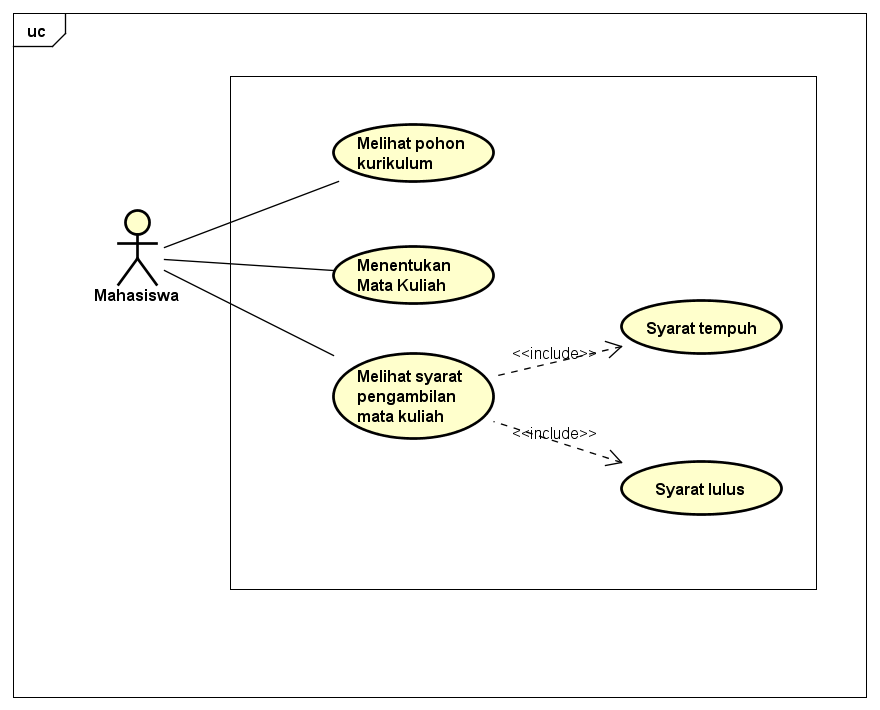
\includegraphics[scale = 0.5]{UseCasePohon.png}
		\caption{Use Case Pohon Kurikulum}
		\label{fig: Use Case Pohon Kurikulum}
\end{figure}	

Berikut keterangan dan skenario dari Gambar \ref{fig: Use Case Pohon Kurikulum}:
\begin{enumerate}
\item Nama \textit{use case} : Melihat Pohon Kurikulum \\
	  Aktor : Mahasiswa 
	  Deskripsi :  Aktor melihat isi pohon kurikulum 
	  Prakondisi : Aktor belum mengetahui pohon kurikulum baru 
	  Skenario normal : Aktor melihat pohon kurikulum
	  Eksepsi : Aktor telah mengetahui pohon kurikulum yang di pakai di kurikulum baru
	  
\item Nama \textit{use case} : Menentukan Mata Kuliah \\
	  Aktor : Mahasiswa 
	  Deskripsi :  Aktor menentukan mata kuliah yang akan diambil 
	  Prakondisi : Aktor sudah mengetahui pohon kurikulum dari kurikulum baru
	  Skenario normal :
	  \begin{enumerate}
	  \item Aktor melihat pohon kurikulum
	  \item Aktor mengetahui mata kuliah yang akan diambil
	  \end{enumerate}
	  Eksepsi : Aktor dapat menentukan mata kuliah yang akan diambil setelah melihat pohon kurikulum
	  
\item Nama \textit{use case} : Melihat Syarat Pengambilan Mata Kuliah \\
	  Aktor : Mahasiswa 
	  Deskripsi :  Aktor melihat syarat pengambilan mata kuliah
	  Prakondisi : Aktor sudah menentukan mata kuliah apa yang akan diambil
	  Skenario normal : 
	  \begin{enumerate}
	  \item Aktor melihat pohon kurikulum
	  \item Aktor mengetahui mata kuliah yang akan diambil
	  \item Aktor melihat syarat pada mata kuliah yang akan diambil
	  \end{enumerate}
	  Eksepsi : Aktor mengetahui syarat pada mata kuliah yang akan diambil
	  
\item Nama \textit{use case} : Syarat Tempuh \\
	  Aktor : Mahasiswa \\
	  Deskripsi :  Aktor melihat syarat mata kuliah
	  Prakondisi : Aktor belum mengetahui syarat untuk mengambil mata kuliah yang diinginkan
	  Skenario normal : Aktor melihat syarat pada mata kuliah yang diinginkan
	  Eksepsi : Aktor telah mengetahui mata kuliah yang akan diambil memiliki syarat tempuh
	 
\item Nama \textit{use case} : Syarat Lulus \\
	  Aktor : Mahasiswa \\
	  Deskripsi :  Aktor melihat syarat mata kuliah
	  Prakondisi : Aktor belum mengetahui syarat untuk mengambil mata kuliah yang diinginkan
	  Skenario normal : Aktor melihat syarat pada mata kuliah yang diinginkan
	  Eksepsi : Aktor telah mengetahui mata kuliah yang akan diambil memiliki syarat lulus
\end{enumerate}


